% -*- TeX-master: "../paper_notes.tex" -*-

\section{Capacitive loss induced during JJ fabrication}
\label{sec:capac-loss-induc}

\begin{framed}\noindent
  The goal  is to  improve the time  $ T_{1} $  of fabricated  qubits.  They are  usually much
  shorter than the time  constant of the resonators they attach to, and  thus are the limiting
  factor.

  When making a JJ, you go through the process of
  \begin{enumerate}
  \item Rinse  wafer in sonic acetone,  and rinse in deionized  water \ira dip wafer  in HF to
    remove oxide layer;
  \item Blow in nitrogen and deposit 100\,nm of Al;
  \item     \red{Optical    lithography}     to    define     resonators    and     capacitors
    ($ \ge \iunitMixed{10}{\mu}{m} $) \ra develop resist and develop Al not covered by resist with
    etching solution;
  \item  \red{EBL  lithography}  for  JJ  ($  100  \iunit{}{nm}  $)  \ira  \red{\textbf{before
        depositing ion mill the surface to etch away  AlOx on resonator, in order to make good
        contact between it and the JJ}};
  \end{enumerate}

  \noindent  This last  process leaves  behind  a dielectric,  which  causes a  lot of  losses
  (microwaves  loose energy  in  these regions).   \red{So  while the  resonators  have a  low
    decoherence rate, qubits have a high one}
\end{framed}

\begin{figure}[h]
  \centering 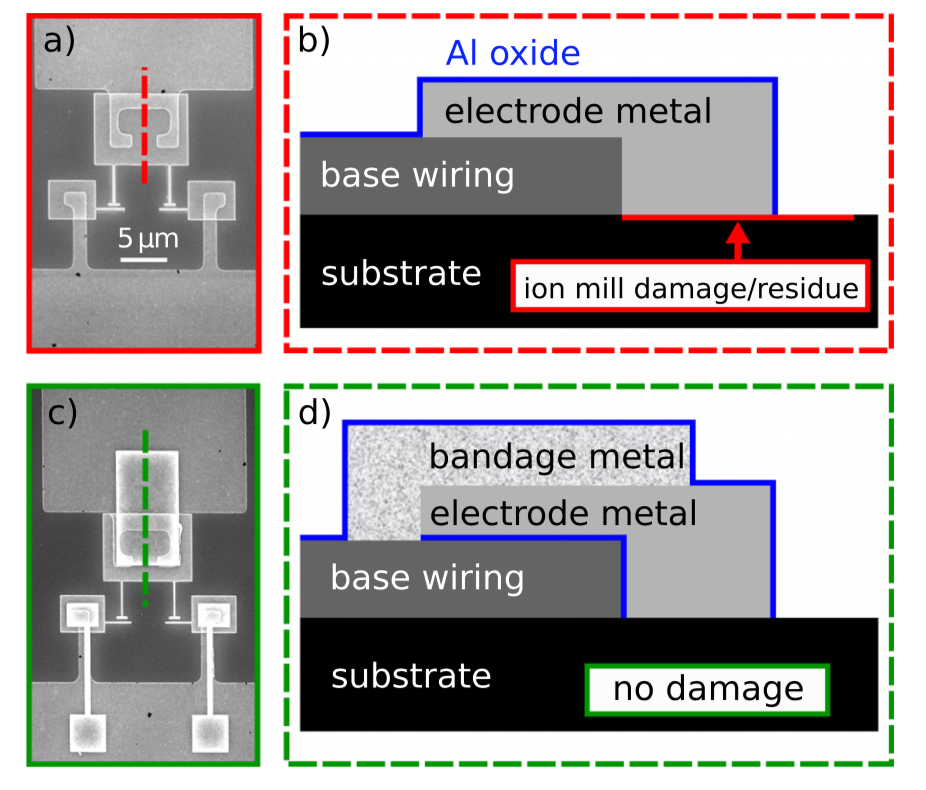
\includegraphics[height=6cm]{dunsworth1}
  \caption{\small b - Damaging  due to milling of surface to remove  oxide between base wiring
    and electrode metal. d - new technology involves depositing electrode metal first and them
    milling the whole  surface. There is no  milling under the electrode metal,  while the top
    oxide layers  are removed.  A bandage  metal slapped  on top  gives the  secret connection
    between the two.}
  \label{fig:dunsworth1.png}
\end{figure}

\subsection{Testing losses}
\label{sec:testing-losses}

Losses are tested by creating JJ-like structures  on the resonator {without connecting the JJs
  themselves,  Fig.~\ref{fig:dunsworth2}.   This  way  we   isolate  dissipation  due  to  the
  fabrication of JJ, and \textbf{not} the JJ effects.}

\begin{figure}[h]
  \centering 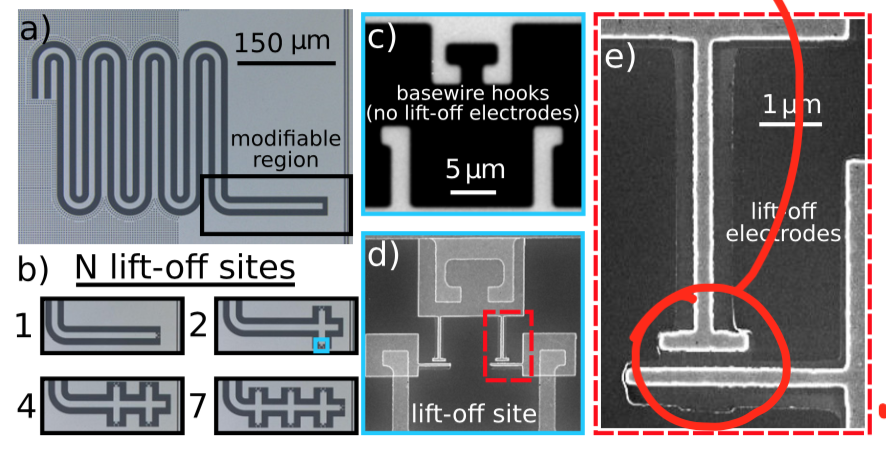
\includegraphics[height=6cm]{dunsworth2}
  \caption{\small JJ structures are created on the  end of the resonator. The focus is looking
    at electrodes (the T shaped things) that connect  JJ to the resonator.  Already, in e), it
    can  be seen  how damage  is done  to  the substrate  in the  ion milling  step, prior  to
    depositing the capacitors.\label{fig:dunsworth2}}
\end{figure}

Resonators are almost ideal, irrelevant of the number of these side ``boxes'' (to which the JJ
are hooked to).  \red{\textbf{As  soon as the JJ structures are placed,  the quality factor of
    the system decreases.}} Aggressive milling of  substrate leads to amorphization, leaving a
3.9\,nm thick layer that will act as the dielectric.

\subsection{New technology}
\label{sec:new-technology}

\paragraph{Wiring}

The way  to counteract  this, is to  deposit the  JJ metal  on top of  the resonator,  with no
milling. \red{\textbf{This  means that at  this stage, there is  an oxide layer  between them,
    preventing a galvanic contact}}.

\paragraph{Bandage}

Next, we use an EBL to expose the JJ and resonator surfaces, in their area of overlap. Now ion
milling is used, to remove  the oxide layer on this overlap, and a  bandage metal is lumped on
top, creating a galvanic contact as in Fig.~\ref{fig:dunsworth1.png}.

\subsection{Result}
\label{sec:result}

A great improvement in the T$_1$ was measured.

\begin{figure}[h]
  \centering 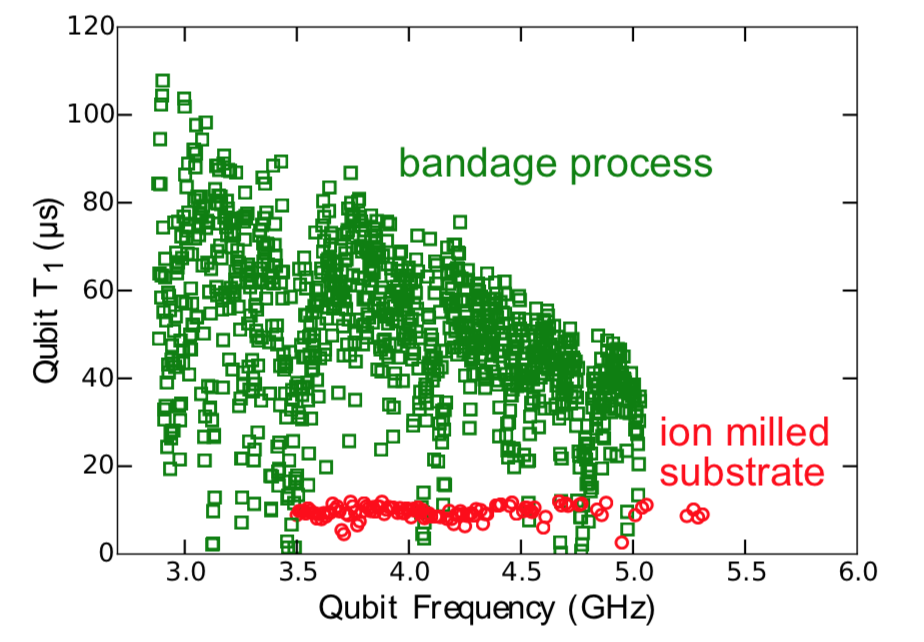
\includegraphics[height=4cm]{dunsworth3}
  \caption{\small Feel the difference\label{fig:dunsworth3}}
\end{figure}
